% Options for packages loaded elsewhere
\PassOptionsToPackage{unicode}{hyperref}
\PassOptionsToPackage{hyphens}{url}
%
\documentclass[
]{article}
\usepackage{amsmath,amssymb}
\usepackage{lmodern}
\usepackage{ifxetex,ifluatex}
\ifnum 0\ifxetex 1\fi\ifluatex 1\fi=0 % if pdftex
  \usepackage[T1]{fontenc}
  \usepackage[utf8]{inputenc}
  \usepackage{textcomp} % provide euro and other symbols
\else % if luatex or xetex
  \usepackage{unicode-math}
  \defaultfontfeatures{Scale=MatchLowercase}
  \defaultfontfeatures[\rmfamily]{Ligatures=TeX,Scale=1}
\fi
% Use upquote if available, for straight quotes in verbatim environments
\IfFileExists{upquote.sty}{\usepackage{upquote}}{}
\IfFileExists{microtype.sty}{% use microtype if available
  \usepackage[]{microtype}
  \UseMicrotypeSet[protrusion]{basicmath} % disable protrusion for tt fonts
}{}
\makeatletter
\@ifundefined{KOMAClassName}{% if non-KOMA class
  \IfFileExists{parskip.sty}{%
    \usepackage{parskip}
  }{% else
    \setlength{\parindent}{0pt}
    \setlength{\parskip}{6pt plus 2pt minus 1pt}}
}{% if KOMA class
  \KOMAoptions{parskip=half}}
\makeatother
\usepackage{xcolor}
\IfFileExists{xurl.sty}{\usepackage{xurl}}{} % add URL line breaks if available
\IfFileExists{bookmark.sty}{\usepackage{bookmark}}{\usepackage{hyperref}}
\hypersetup{
  pdftitle={Pain Reduction Analysis},
  pdfauthor={Rumil Legaspi},
  hidelinks,
  pdfcreator={LaTeX via pandoc}}
\urlstyle{same} % disable monospaced font for URLs
\usepackage[margin=1in]{geometry}
\usepackage{color}
\usepackage{fancyvrb}
\newcommand{\VerbBar}{|}
\newcommand{\VERB}{\Verb[commandchars=\\\{\}]}
\DefineVerbatimEnvironment{Highlighting}{Verbatim}{commandchars=\\\{\}}
% Add ',fontsize=\small' for more characters per line
\usepackage{framed}
\definecolor{shadecolor}{RGB}{248,248,248}
\newenvironment{Shaded}{\begin{snugshade}}{\end{snugshade}}
\newcommand{\AlertTok}[1]{\textcolor[rgb]{0.94,0.16,0.16}{#1}}
\newcommand{\AnnotationTok}[1]{\textcolor[rgb]{0.56,0.35,0.01}{\textbf{\textit{#1}}}}
\newcommand{\AttributeTok}[1]{\textcolor[rgb]{0.77,0.63,0.00}{#1}}
\newcommand{\BaseNTok}[1]{\textcolor[rgb]{0.00,0.00,0.81}{#1}}
\newcommand{\BuiltInTok}[1]{#1}
\newcommand{\CharTok}[1]{\textcolor[rgb]{0.31,0.60,0.02}{#1}}
\newcommand{\CommentTok}[1]{\textcolor[rgb]{0.56,0.35,0.01}{\textit{#1}}}
\newcommand{\CommentVarTok}[1]{\textcolor[rgb]{0.56,0.35,0.01}{\textbf{\textit{#1}}}}
\newcommand{\ConstantTok}[1]{\textcolor[rgb]{0.00,0.00,0.00}{#1}}
\newcommand{\ControlFlowTok}[1]{\textcolor[rgb]{0.13,0.29,0.53}{\textbf{#1}}}
\newcommand{\DataTypeTok}[1]{\textcolor[rgb]{0.13,0.29,0.53}{#1}}
\newcommand{\DecValTok}[1]{\textcolor[rgb]{0.00,0.00,0.81}{#1}}
\newcommand{\DocumentationTok}[1]{\textcolor[rgb]{0.56,0.35,0.01}{\textbf{\textit{#1}}}}
\newcommand{\ErrorTok}[1]{\textcolor[rgb]{0.64,0.00,0.00}{\textbf{#1}}}
\newcommand{\ExtensionTok}[1]{#1}
\newcommand{\FloatTok}[1]{\textcolor[rgb]{0.00,0.00,0.81}{#1}}
\newcommand{\FunctionTok}[1]{\textcolor[rgb]{0.00,0.00,0.00}{#1}}
\newcommand{\ImportTok}[1]{#1}
\newcommand{\InformationTok}[1]{\textcolor[rgb]{0.56,0.35,0.01}{\textbf{\textit{#1}}}}
\newcommand{\KeywordTok}[1]{\textcolor[rgb]{0.13,0.29,0.53}{\textbf{#1}}}
\newcommand{\NormalTok}[1]{#1}
\newcommand{\OperatorTok}[1]{\textcolor[rgb]{0.81,0.36,0.00}{\textbf{#1}}}
\newcommand{\OtherTok}[1]{\textcolor[rgb]{0.56,0.35,0.01}{#1}}
\newcommand{\PreprocessorTok}[1]{\textcolor[rgb]{0.56,0.35,0.01}{\textit{#1}}}
\newcommand{\RegionMarkerTok}[1]{#1}
\newcommand{\SpecialCharTok}[1]{\textcolor[rgb]{0.00,0.00,0.00}{#1}}
\newcommand{\SpecialStringTok}[1]{\textcolor[rgb]{0.31,0.60,0.02}{#1}}
\newcommand{\StringTok}[1]{\textcolor[rgb]{0.31,0.60,0.02}{#1}}
\newcommand{\VariableTok}[1]{\textcolor[rgb]{0.00,0.00,0.00}{#1}}
\newcommand{\VerbatimStringTok}[1]{\textcolor[rgb]{0.31,0.60,0.02}{#1}}
\newcommand{\WarningTok}[1]{\textcolor[rgb]{0.56,0.35,0.01}{\textbf{\textit{#1}}}}
\usepackage{graphicx}
\makeatletter
\def\maxwidth{\ifdim\Gin@nat@width>\linewidth\linewidth\else\Gin@nat@width\fi}
\def\maxheight{\ifdim\Gin@nat@height>\textheight\textheight\else\Gin@nat@height\fi}
\makeatother
% Scale images if necessary, so that they will not overflow the page
% margins by default, and it is still possible to overwrite the defaults
% using explicit options in \includegraphics[width, height, ...]{}
\setkeys{Gin}{width=\maxwidth,height=\maxheight,keepaspectratio}
% Set default figure placement to htbp
\makeatletter
\def\fps@figure{htbp}
\makeatother
\setlength{\emergencystretch}{3em} % prevent overfull lines
\providecommand{\tightlist}{%
  \setlength{\itemsep}{0pt}\setlength{\parskip}{0pt}}
\setcounter{secnumdepth}{-\maxdimen} % remove section numbering
\ifluatex
  \usepackage{selnolig}  % disable illegal ligatures
\fi

\title{Pain Reduction Analysis}
\author{Rumil Legaspi}
\date{8/26/2021}

\begin{document}
\maketitle

\hypertarget{pain-reduction-analysis-project}{%
\section{Pain Reduction Analysis
Project}\label{pain-reduction-analysis-project}}

\hypertarget{introduction}{%
\subsection{Introduction}\label{introduction}}

Pain reduction - the primary efficacy endpoint of the QUEST Study.
Understanding the level of pain reduced holds utmost importance, not
only for the clinical team at NEUROS, but more importantly for the
under-served post-amputee population seeking treatment. In nearing the
end of the study, we have seen an increase in the passing of subjects
within the eligibility phase, specifically, during the saline and
lidocaine injections. This short analysis aims to explore the Saline and
Lidocaine injections of subjects within the years of 2019 to the month
of August 2021, using data extracts derived from the EDC system,
Clindex.

\hypertarget{objectives-and-questions}{%
\section{Objectives and Questions}\label{objectives-and-questions}}

The following are a few questions this analysis seeks to better
understand:

\begin{itemize}
\item
  On average, what is the percent in pain reduction subjects are
  receiving post-saline and lidocaine injection? By Site?
\item
  What do the drops in pain look like? Specifically, how do sites
  compare and look like.
\item
  Based on the passing were seeing how are they passing and if failing
  how are they failing?
\item
  Filter by year 2019,2020, and 2021
\item
  What are the pass rates in 2019-2021 by year (the cut from 23rd aug
  extract)
\item
  how many passed saline, how many passed lidocaines, for all of them
\item
  based on subjects that passed how much on averae did they pass by?
  -Who failed and passed? by year, and in total (all years 2019-2021
  combined)
\item
  then only subjects who passed, I take 0 minute saline mark in those 3
  years and that 0 min column minus 20 minutes to

  \begin{itemize}
  \tightlist
  \item
    see what verage pain decraease is, percentage wise
  \item
    max min, medium,, basic stats
  \item
    highest performing and least performing sites
  \end{itemize}
\end{itemize}

\hypertarget{in-short}{%
\subsection{In short\ldots{}}\label{in-short}}

\begin{itemize}
\tightlist
\item
  sort who passed?
\item
  Analyze pain decrease
\item
  How much are subjects passing by?
\item
  what does the data distribution look like?
\item
  How does it look relative to previous years?
\item
  Any more clues on the increase of injection rates?
\end{itemize}

\hypertarget{loading-in-libraries}{%
\section{Loading in Libraries}\label{loading-in-libraries}}

\begin{verbatim}
## -- Attaching packages --------------------------------------- tidyverse 1.3.1 --
\end{verbatim}

\begin{verbatim}
## v ggplot2 3.3.5     v purrr   0.3.4
## v tibble  3.1.2     v dplyr   1.0.7
## v tidyr   1.1.3     v stringr 1.4.0
## v readr   1.4.0     v forcats 0.5.1
\end{verbatim}

\begin{verbatim}
## -- Conflicts ------------------------------------------ tidyverse_conflicts() --
## x dplyr::filter() masks stats::filter()
## x dplyr::lag()    masks stats::lag()
\end{verbatim}

\begin{verbatim}
## 
## Attaching package: 'lubridate'
\end{verbatim}

\begin{verbatim}
## The following objects are masked from 'package:base':
## 
##     date, intersect, setdiff, union
\end{verbatim}

\begin{verbatim}
## 
## Attaching package: 'cowplot'
\end{verbatim}

\begin{verbatim}
## The following object is masked from 'package:lubridate':
## 
##     stamp
\end{verbatim}

\hypertarget{filepaths}{%
\section{Filepaths}\label{filepaths}}

\begin{Shaded}
\begin{Highlighting}[]
\CommentTok{\#pc \textless{}{-}}
\end{Highlighting}
\end{Shaded}

\hypertarget{importing-data}{%
\section{1. Importing Data}\label{importing-data}}

\begin{Shaded}
\begin{Highlighting}[]
\CommentTok{\# Evaluation Visit}
\NormalTok{eval\_visit }\OtherTok{\textless{}{-}} \FunctionTok{read\_csv}\NormalTok{(}\StringTok{"Data/nm\_evalvis (5).csv"}\NormalTok{, }\AttributeTok{locale =} \FunctionTok{locale}\NormalTok{(}\AttributeTok{encoding =} \StringTok{"Latin1"}\NormalTok{))}
\end{Highlighting}
\end{Shaded}

\begin{verbatim}
## 
## -- Column specification --------------------------------------------------------
## cols(
##   .default = col_character(),
##   KEYID = col_double(),
##   `Injection Evlaution Form Number` = col_double(),
##   Time = col_time(format = ""),
##   `Time of Pain rating` = col_time(format = ""),
##   `Time of saline injection` = col_time(format = ""),
##   `End of Saline Assessment Time` = col_time(format = ""),
##   `Time of lidocaine injection` = col_time(format = ""),
##   `End of Lidocaine Assessment Time` = col_time(format = "")
## )
## i Use `spec()` for the full column specifications.
\end{verbatim}

\begin{Shaded}
\begin{Highlighting}[]
\CommentTok{\#View(nm\_evalvis\_5\_)}

\CommentTok{\# Saline Injections}
\NormalTok{saline\_inj }\OtherTok{\textless{}{-}} \FunctionTok{read\_csv}\NormalTok{(}\StringTok{"Data/nm\_saline.csv"}\NormalTok{)}
\end{Highlighting}
\end{Shaded}

\begin{verbatim}
## 
## -- Column specification --------------------------------------------------------
## cols(
##   KEYID = col_double(),
##   SUB_KEYID = col_double(),
##   CLDV_ROWID = col_double(),
##   `Unique Subject ID` = col_character(),
##   `0 min` = col_double(),
##   `+ 5 min` = col_double(),
##   `+ 10 min` = col_double(),
##   `+ 15 min` = col_double(),
##   `+ 20 min` = col_double()
## )
\end{verbatim}

\begin{Shaded}
\begin{Highlighting}[]
\CommentTok{\#View(saline\_inj)}

\CommentTok{\# Lidocaine Injections}
\NormalTok{lidocaine\_inj }\OtherTok{\textless{}{-}} \FunctionTok{read\_csv}\NormalTok{(}\StringTok{"Data/nm\_lidocain.csv"}\NormalTok{)}
\end{Highlighting}
\end{Shaded}

\begin{verbatim}
## 
## -- Column specification --------------------------------------------------------
## cols(
##   KEYID = col_double(),
##   SUB_KEYID = col_double(),
##   CLDV_ROWID = col_double(),
##   `Unique Subject ID` = col_character(),
##   `0 min` = col_double(),
##   `+ 5 min` = col_double(),
##   `+ 10 min` = col_double(),
##   `+ 15 min` = col_double(),
##   `+ 20 min` = col_double()
## )
\end{verbatim}

\begin{Shaded}
\begin{Highlighting}[]
\CommentTok{\#View(lidocaine\_inj)}
\end{Highlighting}
\end{Shaded}

\hypertarget{joining-datasets}{%
\section{Joining Datasets}\label{joining-datasets}}

\begin{Shaded}
\begin{Highlighting}[]
\CommentTok{\# 1. left Joining saline and Lidocaine datasets first}

\FunctionTok{glimpse}\NormalTok{(saline\_inj)}
\end{Highlighting}
\end{Shaded}

\begin{verbatim}
## Rows: 354
## Columns: 9
## $ KEYID               <dbl> 26171, 32171, 140171, 147171, 170171, 200171, 2241~
## $ SUB_KEYID           <dbl> 1, 1, 1, 1, 1, 1, 1, 1, 1, 1, 1, 1, 1, 1, 1, 1, 1,~
## $ CLDV_ROWID          <dbl> 1, 1, 1, 1, 1, 1, 1, 1, 1, 1, 1, 1, 1, 1, 1, 1, 1,~
## $ `Unique Subject ID` <chr> "05-001", "01-001", "05-002", "01-002", "01-003", ~
## $ `0 min`             <dbl> 5, 8, 6, 5, 7, 8, 8, 6, 7, 7, 7, 6, 8, 7, 5, 7, 6,~
## $ `+ 5 min`           <dbl> 0, 8, 6, 5, 5, 8, 7, 6, 5, 7, 7, 5, 5, 6, 5, 7, 6,~
## $ `+ 10 min`          <dbl> 5, 8, 6, 5, 6, 8, 6, 6, 5, 7, 6, 5, 5, 6, 5, 7, 6,~
## $ `+ 15 min`          <dbl> 5, 8, 6, 5, 6, 8, 7, 6, 6, 7, 2, 5, 7, 6, 3, 7, 6,~
## $ `+ 20 min`          <dbl> 5, 8, 6, 5, 4, 8, 7, 6, 6, 7, 2, 5, 7, 6, 3, 7, 6,~
\end{verbatim}

\begin{Shaded}
\begin{Highlighting}[]
\FunctionTok{glimpse}\NormalTok{(lidocaine\_inj)}
\end{Highlighting}
\end{Shaded}

\begin{verbatim}
## Rows: 354
## Columns: 9
## $ KEYID               <dbl> 26171, 32171, 140171, 147171, 170171, 200171, 2241~
## $ SUB_KEYID           <dbl> 1, 1, 1, 1, 1, 1, 1, 1, 1, 1, 1, 1, 1, 1, 1, 1, 1,~
## $ CLDV_ROWID          <dbl> 1, 1, 1, 1, 1, 1, 1, 1, 1, 1, 1, 1, 1, 1, 1, 1, 1,~
## $ `Unique Subject ID` <chr> "05-001", "01-001", "05-002", "01-002", "01-003", ~
## $ `0 min`             <dbl> 7, 8, 6, 5, 7, 8, 8, 6, 6, 7, NA, 7, 7, 7, NA, 7, ~
## $ `+ 5 min`           <dbl> 5, 0, 4, 4, 2, 8, 6, 5, 4, 6, NA, 4, 4, 5, NA, 6, ~
## $ `+ 10 min`          <dbl> 3, 0, 4, 4, 3, 7, 5, 5, 4, 6, NA, NA, 4, 4, NA, 5,~
## $ `+ 15 min`          <dbl> 0, 0, 0, 3, 3, 6, 3, 5, 3, 6, NA, NA, 5, 3, NA, 1,~
## $ `+ 20 min`          <dbl> 0, 0, 0, 3, 3, 6, 4, 4, 3, 5, NA, NA, 5, 3, NA, 1,~
\end{verbatim}

\begin{Shaded}
\begin{Highlighting}[]
\NormalTok{sal\_lido\_join }\OtherTok{\textless{}{-}} \FunctionTok{left\_join}\NormalTok{(saline\_inj, lidocaine\_inj, }\AttributeTok{by =} \StringTok{"KEYID"}\NormalTok{)}

\CommentTok{\# 2. left joining saline and lido dataset with evaluation visit dataset}

\NormalTok{inj\_data }\OtherTok{\textless{}{-}} \FunctionTok{left\_join}\NormalTok{(sal\_lido\_join, eval\_visit, }\AttributeTok{by =} \StringTok{"KEYID"}\NormalTok{) }
\end{Highlighting}
\end{Shaded}

\hypertarget{data-cleaning}{%
\section{2. Data Cleaning}\label{data-cleaning}}

\begin{Shaded}
\begin{Highlighting}[]
\CommentTok{\# Selecting \& renaming Columns}
\NormalTok{cleaning\_inj\_data }\OtherTok{\textless{}{-}}\NormalTok{ inj\_data }\SpecialCharTok{\%\textgreater{}\%} 
  \FunctionTok{rename}\NormalTok{(}\AttributeTok{key\_id              =}\NormalTok{ KEYID,}
         \AttributeTok{site                =} \StringTok{\textasciigrave{}}\AttributeTok{Site \#}\StringTok{\textasciigrave{}}\NormalTok{,}
         \AttributeTok{subj\_id             =} \StringTok{\textasciigrave{}}\AttributeTok{SUB\_KEYID.x}\StringTok{\textasciigrave{}}\NormalTok{,}
         \AttributeTok{visit\_date          =} \StringTok{\textasciigrave{}}\AttributeTok{Date of visit}\StringTok{\textasciigrave{}}\NormalTok{,}
         \AttributeTok{sal\_0min            =} \StringTok{\textasciigrave{}}\AttributeTok{0 min.x}\StringTok{\textasciigrave{}}\NormalTok{,}
         \AttributeTok{sal\_5min            =} \StringTok{\textasciigrave{}}\AttributeTok{+ 5 min.x}\StringTok{\textasciigrave{}}\NormalTok{,}
         \AttributeTok{sal\_10min           =} \StringTok{\textasciigrave{}}\AttributeTok{+ 10 min.x}\StringTok{\textasciigrave{}}\NormalTok{,}
         \AttributeTok{sal\_15min           =} \StringTok{\textasciigrave{}}\AttributeTok{+ 15 min.x}\StringTok{\textasciigrave{}}\NormalTok{,}
         \AttributeTok{sal\_20min           =} \StringTok{\textasciigrave{}}\AttributeTok{+ 20 min.x}\StringTok{\textasciigrave{}}\NormalTok{,}
         \AttributeTok{lido\_0min           =} \StringTok{\textasciigrave{}}\AttributeTok{0 min.y}\StringTok{\textasciigrave{}}\NormalTok{,}
         \AttributeTok{lido\_5min           =} \StringTok{\textasciigrave{}}\AttributeTok{+ 5 min.y}\StringTok{\textasciigrave{}}\NormalTok{,}
         \AttributeTok{lido\_10min          =} \StringTok{\textasciigrave{}}\AttributeTok{+ 10 min.y}\StringTok{\textasciigrave{}}\NormalTok{,}
         \AttributeTok{lido\_15min          =} \StringTok{\textasciigrave{}}\AttributeTok{+ 15 min.y}\StringTok{\textasciigrave{}}\NormalTok{,}
         \AttributeTok{lido\_20min          =} \StringTok{\textasciigrave{}}\AttributeTok{+ 20 min.y}\StringTok{\textasciigrave{}}\NormalTok{,}
         \AttributeTok{inj\_eval\_num        =} \StringTok{\textasciigrave{}}\AttributeTok{Injection Evlaution Form Number}\StringTok{\textasciigrave{}}\NormalTok{,}
         \AttributeTok{meds\_today          =} \StringTok{\textasciigrave{}}\AttributeTok{N/A, None today}\StringTok{\textasciigrave{}}\NormalTok{,}
         \AttributeTok{med\_name            =}\NormalTok{ Name,}
         \AttributeTok{med\_dose            =}\NormalTok{ Dose,}
         \AttributeTok{med\_time            =}\NormalTok{ Time,}
         \AttributeTok{time\_intl\_pain\_lvl  =} \StringTok{\textasciigrave{}}\AttributeTok{Time of Pain rating}\StringTok{\textasciigrave{}}\NormalTok{,}
         \AttributeTok{intl\_pain\_lvl       =} \StringTok{\textasciigrave{}}\AttributeTok{What is subject\textless{}U+0092\textgreater{}s Overall limb pain right now?}\StringTok{\textasciigrave{}}\NormalTok{,}
         \AttributeTok{sal\_inj\_not\_done    =} \StringTok{\textasciigrave{}}\AttributeTok{Saline Injection Not Done}\StringTok{\textasciigrave{}}\NormalTok{ ,}
         \AttributeTok{inj\_location        =} \StringTok{\textasciigrave{}}\AttributeTok{Target of injection}\StringTok{\textasciigrave{}}\NormalTok{,}
         \AttributeTok{sal\_inj\_start\_time  =} \StringTok{\textasciigrave{}}\AttributeTok{Time of saline injection}\StringTok{\textasciigrave{}}\NormalTok{,}
         \AttributeTok{sal\_inj\_end\_time    =} \StringTok{\textasciigrave{}}\AttributeTok{End of Saline Assessment Time}\StringTok{\textasciigrave{}}\NormalTok{,}
         \AttributeTok{sal\_eval\_outcome    =} \StringTok{\textasciigrave{}}\AttributeTok{Saline Injection Outcome?}\StringTok{\textasciigrave{}}\NormalTok{,}
         \AttributeTok{lido\_inj\_start\_time =} \StringTok{\textasciigrave{}}\AttributeTok{Time of lidocaine injection}\StringTok{\textasciigrave{}}\NormalTok{,}
         \AttributeTok{lido\_inj\_end\_time   =} \StringTok{\textasciigrave{}}\AttributeTok{End of Lidocaine Assessment Time}\StringTok{\textasciigrave{}}\NormalTok{,}
         \AttributeTok{lido\_eval\_outcome   =} \StringTok{\textasciigrave{}}\AttributeTok{Lidocaine Injection Outcome}\StringTok{\textasciigrave{}} 
         
\NormalTok{         )}
\end{Highlighting}
\end{Shaded}

Dropping and Rearranging Columns

\begin{Shaded}
\begin{Highlighting}[]
\CommentTok{\# Checking Column Indexes}
\FunctionTok{colnames}\NormalTok{(cleaning\_inj\_data)}
\end{Highlighting}
\end{Shaded}

\begin{verbatim}
##  [1] "key_id"                                                                  
##  [2] "subj_id"                                                                 
##  [3] "CLDV_ROWID.x"                                                            
##  [4] "Unique Subject ID.x"                                                     
##  [5] "sal_0min"                                                                
##  [6] "sal_5min"                                                                
##  [7] "sal_10min"                                                               
##  [8] "sal_15min"                                                               
##  [9] "sal_20min"                                                               
## [10] "SUB_KEYID.y"                                                             
## [11] "CLDV_ROWID.y"                                                            
## [12] "Unique Subject ID.y"                                                     
## [13] "lido_0min"                                                               
## [14] "lido_5min"                                                               
## [15] "lido_10min"                                                              
## [16] "lido_15min"                                                              
## [17] "lido_20min"                                                              
## [18] "site"                                                                    
## [19] "Unique Subject ID"                                                       
## [20] "inj_eval_num"                                                            
## [21] "visit_date"                                                              
## [22] "meds_today"                                                              
## [23] "med_name"                                                                
## [24] "med_dose"                                                                
## [25] "med_time"                                                                
## [26] "time_intl_pain_lvl"                                                      
## [27] "intl_pain_lvl"                                                           
## [28] "What is subject<U+0092>s Phantom pain right now?"                        
## [29] "What is subject<U+0092>s Stump pain right now?"                          
## [30] "sal_inj_not_done"                                                        
## [31] "inj_location"                                                            
## [32] "sal_inj_start_time"                                                      
## [33] "What is subject<U+0092>s Phantom pain after saline injection?"           
## [34] "What is subject<U+0092>s Stump pain after saline injection?"             
## [35] "sal_inj_end_time"                                                        
## [36] "sal_eval_outcome"                                                        
## [37] "Lidocaine Injection Not Done"                                            
## [38] "lido_inj_start_time"                                                     
## [39] "What is subject<U+0092>s Phantom pain right now after lidocaine injection?"
## [40] "What is subject<U+0092>s Stump pain right now after lidocaine injection?"
## [41] "lido_inj_end_time"                                                       
## [42] "Injection Evaluation Outcome"                                            
## [43] "What is the subject s Overall limb pain right now?"                      
## [44] "What is he subject s Overal limb pain right now?"                        
## [45] "lido_eval_outcome"
\end{verbatim}

\begin{Shaded}
\begin{Highlighting}[]
\CommentTok{\#Dropping by col index}
\NormalTok{cleaning\_inj\_data }\OtherTok{\textless{}{-}}\NormalTok{ cleaning\_inj\_data[}\SpecialCharTok{{-}}\FunctionTok{c}\NormalTok{(}\DecValTok{2}\NormalTok{, }\DecValTok{3}\NormalTok{, }\DecValTok{4}\NormalTok{, }\DecValTok{10}\NormalTok{, }\DecValTok{11}\NormalTok{, }\DecValTok{12}\NormalTok{, }\DecValTok{28}\NormalTok{, }\DecValTok{29}\NormalTok{, }\DecValTok{33}\NormalTok{, }\DecValTok{34}\NormalTok{, }\DecValTok{39}\NormalTok{, }\DecValTok{40}\NormalTok{, }\DecValTok{43}\NormalTok{, }\DecValTok{44}\NormalTok{)] }\SpecialCharTok{\%\textgreater{}\%} \FunctionTok{rename}\NormalTok{(}\AttributeTok{subj\_id =} \StringTok{\textasciigrave{}}\AttributeTok{Unique Subject ID}\StringTok{\textasciigrave{}}\NormalTok{,}
                \AttributeTok{lidocaine\_injection\_not\_done =} \StringTok{\textasciigrave{}}\AttributeTok{Lidocaine Injection Not Done}\StringTok{\textasciigrave{}}\NormalTok{,}
                \AttributeTok{injection\_evaluation\_outcome =} \StringTok{\textasciigrave{}}\AttributeTok{Injection Evaluation Outcome}\StringTok{\textasciigrave{}}
\NormalTok{                ) }

\CommentTok{\#Rearranging Columns}
\NormalTok{cleaning\_inj\_data }\OtherTok{\textless{}{-}}\NormalTok{ cleaning\_inj\_data }\SpecialCharTok{\%\textgreater{}\%} 
  \FunctionTok{relocate}\NormalTok{(site, subj\_id, }\AttributeTok{.after =}\NormalTok{ key\_id)}
\end{Highlighting}
\end{Shaded}

\hypertarget{needs-work}{%
\section{Needs Work}\label{needs-work}}

\begin{Shaded}
\begin{Highlighting}[]
\NormalTok{cleaning\_inj\_data }\SpecialCharTok{\%\textgreater{}\%} \FunctionTok{glimpse}\NormalTok{()}
\end{Highlighting}
\end{Shaded}

\begin{verbatim}
## Rows: 354
## Columns: 31
## $ key_id                       <dbl> 26171, 32171, 140171, 147171, 170171, 200~
## $ site                         <chr> "5 - Cleveland Clinic Pain Management", "~
## $ subj_id                      <chr> "05-001", "01-001", "05-002", "01-002", "~
## $ sal_0min                     <dbl> 5, 8, 6, 5, 7, 8, 8, 6, 7, 7, 7, 6, 8, 7,~
## $ sal_5min                     <dbl> 0, 8, 6, 5, 5, 8, 7, 6, 5, 7, 7, 5, 5, 6,~
## $ sal_10min                    <dbl> 5, 8, 6, 5, 6, 8, 6, 6, 5, 7, 6, 5, 5, 6,~
## $ sal_15min                    <dbl> 5, 8, 6, 5, 6, 8, 7, 6, 6, 7, 2, 5, 7, 6,~
## $ sal_20min                    <dbl> 5, 8, 6, 5, 4, 8, 7, 6, 6, 7, 2, 5, 7, 6,~
## $ lido_0min                    <dbl> 7, 8, 6, 5, 7, 8, 8, 6, 6, 7, NA, 7, 7, 7~
## $ lido_5min                    <dbl> 5, 0, 4, 4, 2, 8, 6, 5, 4, 6, NA, 4, 4, 5~
## $ lido_10min                   <dbl> 3, 0, 4, 4, 3, 7, 5, 5, 4, 6, NA, NA, 4, ~
## $ lido_15min                   <dbl> 0, 0, 0, 3, 3, 6, 3, 5, 3, 6, NA, NA, 5, ~
## $ lido_20min                   <dbl> 0, 0, 0, 3, 3, 6, 4, 4, 3, 5, NA, NA, 5, ~
## $ inj_eval_num                 <dbl> 1, 1, 1, 1, 1, 1, 1, 1, 1, 1, 1, 1, 2, 1,~
## $ visit_date                   <chr> "12/9/2014", "10/27/2014", "1/6/2015", "1~
## $ meds_today                   <chr> "1 - Yes", "1 - Yes", "1 - Yes", "1 - Yes~
## $ med_name                     <chr> NA, NA, NA, NA, NA, NA, NA, NA, NA, NA, N~
## $ med_dose                     <chr> NA, NA, NA, NA, NA, NA, NA, NA, NA, NA, N~
## $ med_time                     <time>       NA,       NA,       NA,       NA, ~
## $ time_intl_pain_lvl           <time> 12:27:00, 11:07:00, 10:51:00, 08:35:00, ~
## $ intl_pain_lvl                <chr> "118173 - 5", "121173 - 8", "120173 - 7",~
## $ sal_inj_not_done             <chr> NA, "2 - No", NA, NA, NA, NA, NA, NA, NA,~
## $ inj_location                 <chr> "181173 - Bifurcation of Tibial and Commo~
## $ sal_inj_start_time           <time> 12:41:00, 11:47:00, 11:35:00, 10:07:00, ~
## $ sal_inj_end_time             <time> 13:03:00, 12:07:00, 11:55:00, 10:33:00, ~
## $ sal_eval_outcome             <chr> "175173 - Pass", "175173 - Pass", "175173~
## $ lidocaine_injection_not_done <chr> NA, NA, NA, NA, NA, NA, NA, NA, NA, NA, "~
## $ lido_inj_start_time          <time> 13:12:00, 12:16:00, 12:15:00, 11:05:00, ~
## $ lido_inj_end_time            <time> 14:00:00, 12:37:00, 12:35:00, 11:30:00, ~
## $ injection_evaluation_outcome <chr> "173173 - Pass (pain reduction >= 50%)", ~
## $ lido_eval_outcome            <chr> NA, NA, NA, NA, NA, NA, NA, NA, NA, NA, N~
\end{verbatim}

\begin{Shaded}
\begin{Highlighting}[]
\CommentTok{\#Changing Data Types}

\NormalTok{new\_cleaned\_inj\_data }\OtherTok{\textless{}{-}}\NormalTok{ cleaning\_inj\_data }\SpecialCharTok{\%\textgreater{}\%} 
  
  \FunctionTok{mutate}\NormalTok{(}\AttributeTok{visit\_date =} \FunctionTok{as.Date}\NormalTok{(}\FunctionTok{as.character}\NormalTok{(cleaning\_inj\_data}\SpecialCharTok{$}\NormalTok{visit\_date), }\StringTok{"\%m/\%d/\%y"}\NormalTok{, }\AttributeTok{tz =} \StringTok{"UTC"}\NormalTok{))}
\NormalTok{?as.Date}
\end{Highlighting}
\end{Shaded}

\begin{verbatim}
## starting httpd help server ... done
\end{verbatim}

\begin{Shaded}
\begin{Highlighting}[]
  \CommentTok{\#test \textless{}{-} cleaning\_inj\_data \%\textgreater{}\% as.Date(cleaning\_inj\_data$visit\_date, format = "\%m/\%d/\%y")}
\end{Highlighting}
\end{Shaded}

A Quick Distribution of our Variables

\begin{Shaded}
\begin{Highlighting}[]
\NormalTok{Inj\_data\_plots }\OtherTok{\textless{}{-}}\NormalTok{ new\_cleaned\_inj\_data }\SpecialCharTok{\%\textgreater{}\%}
  \FunctionTok{keep}\NormalTok{(is.numeric) }\SpecialCharTok{\%\textgreater{}\%}                       \CommentTok{\# Using numeric columns}
  \FunctionTok{gather}\NormalTok{() }\SpecialCharTok{\%\textgreater{}\%}                                
  \FunctionTok{ggplot}\NormalTok{(}\FunctionTok{aes}\NormalTok{(value)) }\SpecialCharTok{+}                       \CommentTok{\#plotting}
    \FunctionTok{facet\_wrap}\NormalTok{(}\SpecialCharTok{\textasciitilde{}}\NormalTok{ key, }\AttributeTok{scales =} \StringTok{"free"}\NormalTok{) }\SpecialCharTok{+}
    \FunctionTok{geom\_density}\NormalTok{()                         }\CommentTok{\#try geom\_density/histo}
\NormalTok{Inj\_data\_plots}
\end{Highlighting}
\end{Shaded}

\begin{verbatim}
## Warning: Removed 361 rows containing non-finite values (stat_density).
\end{verbatim}

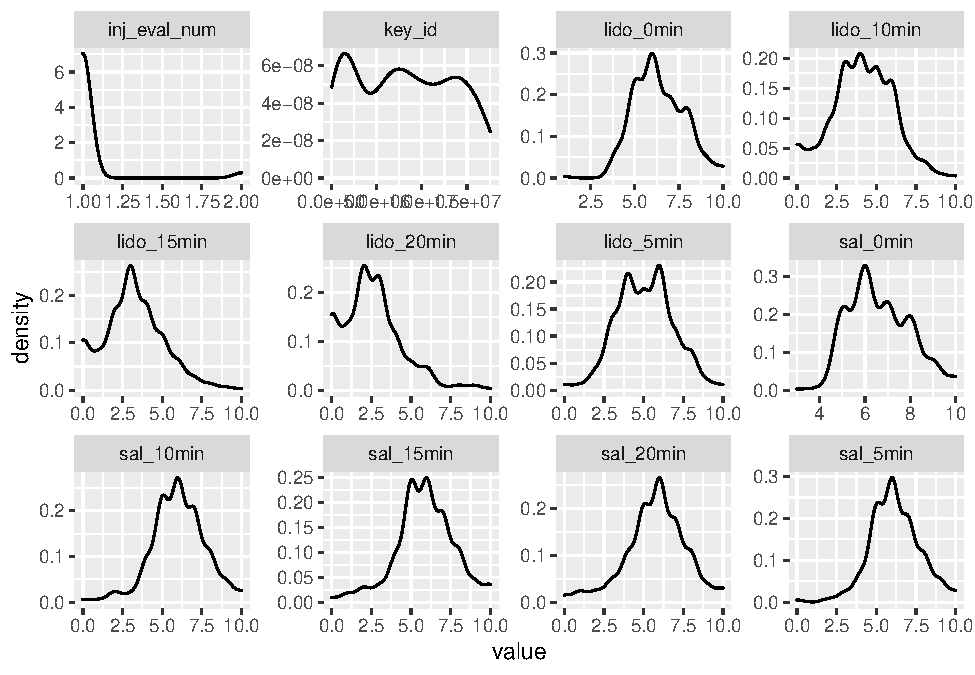
\includegraphics{Painreduction_files/figure-latex/unnamed-chunk-8-1.pdf}

Correlations

\begin{Shaded}
\begin{Highlighting}[]
\CommentTok{\# install.packages("corrr")}
\CommentTok{\# install.packages("corrplot")}
\FunctionTok{library}\NormalTok{(corrplot)}
\end{Highlighting}
\end{Shaded}

\begin{verbatim}
## Warning: package 'corrplot' was built under R version 4.1.1
\end{verbatim}

\begin{verbatim}
## corrplot 0.90 loaded
\end{verbatim}

\begin{Shaded}
\begin{Highlighting}[]
\FunctionTok{library}\NormalTok{(corrr)}
\end{Highlighting}
\end{Shaded}

\begin{verbatim}
## Warning: package 'corrr' was built under R version 4.1.1
\end{verbatim}

\begin{Shaded}
\begin{Highlighting}[]
\NormalTok{Inj\_data\_corr }\OtherTok{\textless{}{-}}\NormalTok{ new\_cleaned\_inj\_data }\SpecialCharTok{\%\textgreater{}\%}
  \FunctionTok{keep}\NormalTok{(is.numeric) }\SpecialCharTok{\%\textgreater{}\%}                       \CommentTok{\# Using numeric columns}
   \FunctionTok{correlate}\NormalTok{() }\SpecialCharTok{\%\textgreater{}\%} \FunctionTok{fashion}\NormalTok{()}
\end{Highlighting}
\end{Shaded}

\begin{verbatim}
## 
## Correlation method: 'pearson'
## Missing treated using: 'pairwise.complete.obs'
\end{verbatim}

\begin{Shaded}
\begin{Highlighting}[]
\NormalTok{Inj\_data\_corr}
\end{Highlighting}
\end{Shaded}

\begin{verbatim}
##            term key_id sal_0min sal_5min sal_10min sal_15min sal_20min
## 1        key_id             .02      .05       .07       .10       .11
## 2      sal_0min    .02               .74       .71       .62       .57
## 3      sal_5min    .05      .74                .88       .77       .72
## 4     sal_10min    .07      .71      .88                 .90       .85
## 5     sal_15min    .10      .62      .77       .90                 .94
## 6     sal_20min    .11      .57      .72       .85       .94          
## 7     lido_0min   -.01      .74      .71       .81       .82       .87
## 8     lido_5min    .08      .53      .54       .62       .62       .65
## 9    lido_10min    .04      .40      .42       .47       .49       .52
## 10   lido_15min    .01      .30      .34       .36       .37       .41
## 11   lido_20min   -.08      .29      .27       .30       .31       .35
## 12 inj_eval_num   -.14      .01     -.03      -.07      -.07      -.08
##    lido_0min lido_5min lido_10min lido_15min lido_20min inj_eval_num
## 1       -.01       .08        .04        .01       -.08         -.14
## 2        .74       .53        .40        .30        .29          .01
## 3        .71       .54        .42        .34        .27         -.03
## 4        .81       .62        .47        .36        .30         -.07
## 5        .82       .62        .49        .37        .31         -.07
## 6        .87       .65        .52        .41        .35         -.08
## 7                  .65        .51        .38        .33          .00
## 8        .65                  .83        .65        .57          .03
## 9        .51       .83                   .84        .76          .01
## 10       .38       .65        .84                   .86          .04
## 11       .33       .57        .76        .86                     .02
## 12       .00       .03        .01        .04        .02
\end{verbatim}

\begin{Shaded}
\begin{Highlighting}[]
\NormalTok{num\_inj\_data }\OtherTok{\textless{}{-}}\NormalTok{ new\_cleaned\_inj\_data }\SpecialCharTok{\%\textgreater{}\%}
  \FunctionTok{keep}\NormalTok{(is.numeric) }\SpecialCharTok{\%\textgreater{}\%} \FunctionTok{subset}\NormalTok{(}\AttributeTok{select =} \SpecialCharTok{{-}}\FunctionTok{c}\NormalTok{(key\_id))}

\FunctionTok{cor}\NormalTok{(num\_inj\_data)}
\end{Highlighting}
\end{Shaded}

\begin{verbatim}
##              sal_0min sal_5min sal_10min sal_15min sal_20min lido_0min
## sal_0min            1       NA        NA        NA        NA        NA
## sal_5min           NA        1        NA        NA        NA        NA
## sal_10min          NA       NA         1        NA        NA        NA
## sal_15min          NA       NA        NA         1        NA        NA
## sal_20min          NA       NA        NA        NA         1        NA
## lido_0min          NA       NA        NA        NA        NA         1
## lido_5min          NA       NA        NA        NA        NA        NA
## lido_10min         NA       NA        NA        NA        NA        NA
## lido_15min         NA       NA        NA        NA        NA        NA
## lido_20min         NA       NA        NA        NA        NA        NA
## inj_eval_num       NA       NA        NA        NA        NA        NA
##              lido_5min lido_10min lido_15min lido_20min inj_eval_num
## sal_0min            NA         NA         NA         NA           NA
## sal_5min            NA         NA         NA         NA           NA
## sal_10min           NA         NA         NA         NA           NA
## sal_15min           NA         NA         NA         NA           NA
## sal_20min           NA         NA         NA         NA           NA
## lido_0min           NA         NA         NA         NA           NA
## lido_5min            1         NA         NA         NA           NA
## lido_10min          NA          1         NA         NA           NA
## lido_15min          NA         NA          1         NA           NA
## lido_20min          NA         NA         NA          1           NA
## inj_eval_num        NA         NA         NA         NA            1
\end{verbatim}

\begin{Shaded}
\begin{Highlighting}[]
\CommentTok{\# matrix\_num\_inj\_data \textless{}{-} as.matrix(as.data.frame(num\_inj\_data))}
\CommentTok{\# \# }
\CommentTok{\# corrplot(matrix\_num\_inj\_data,  method = "number")}
\CommentTok{\# \# }
\CommentTok{\# corrplot(cor(num\_inj\_data))}
\CommentTok{\# }
\CommentTok{\# pretty\_data\_corr \textless{}{-} ggcorrplot( hc.order = TRUE, type = "lower", lab = TRUE,}
\CommentTok{\#                                outline.col = "white",}
\CommentTok{\#                                ggtheme     = ggplot2::theme\_gray,}
\CommentTok{\#                                colors      = c("\#6D9EC1", "white", "\#E46726"))}
\CommentTok{\# pretty\_data\_corr}
\CommentTok{\# }
\CommentTok{\# }
\CommentTok{\# table(new\_cleaned\_inj\_data$lido\_eval\_outcome, new\_cleaned\_inj\_data$inj\_location)}
\CommentTok{\# ggplot(new\_cleaned\_inj\_data, aes(x = inj\_location, fill = lido\_eval\_outcome)) + geom\_bar()}
\CommentTok{\# }
\CommentTok{\# ggplot(new\_cleaned\_inj\_data, aes(x = lido\_eval\_outcome, fill = inj\_location)) + geom\_bar()}

\CommentTok{\#x indicating a count variable, and the fill as the category}
\CommentTok{\#Next task is to go back and clean the observations with extra strings and NA\textquotesingle{}s!}
\CommentTok{\#also remove where target location is na and filter the date to captuer 2019{-}aug2021}
\CommentTok{\# understand the NAs}
\end{Highlighting}
\end{Shaded}

\begin{Shaded}
\begin{Highlighting}[]
\FunctionTok{filter}\NormalTok{(new\_cleaned\_inj\_data, visit\_date }\SpecialCharTok{\textgreater{}=} \StringTok{""}\NormalTok{ )}
\end{Highlighting}
\end{Shaded}

\begin{verbatim}
## # A tibble: 0 x 31
## # ... with 31 variables: key_id <dbl>, site <chr>, subj_id <chr>,
## #   sal_0min <dbl>, sal_5min <dbl>, sal_10min <dbl>, sal_15min <dbl>,
## #   sal_20min <dbl>, lido_0min <dbl>, lido_5min <dbl>, lido_10min <dbl>,
## #   lido_15min <dbl>, lido_20min <dbl>, inj_eval_num <dbl>, visit_date <date>,
## #   meds_today <chr>, med_name <chr>, med_dose <chr>, med_time <time>,
## #   time_intl_pain_lvl <time>, intl_pain_lvl <chr>, sal_inj_not_done <chr>,
## #   inj_location <chr>, sal_inj_start_time <time>, sal_inj_end_time <time>,
## #   sal_eval_outcome <chr>, lidocaine_injection_not_done <chr>,
## #   lido_inj_start_time <time>, lido_inj_end_time <time>,
## #   injection_evaluation_outcome <chr>, lido_eval_outcome <chr>
\end{verbatim}

\begin{Shaded}
\begin{Highlighting}[]
\CommentTok{\# ANOVA! to tell if is significant difference in means of dependent variable given different levels of the categorical independent vars or combinations of levels of the independent variables}

\CommentTok{\# new\_cleaned\_inj\_data \textless{}{-} data.frame(new\_cleaned\_inj\_data, stringsAsFactors = FALSE)}
\CommentTok{\# }
\CommentTok{\# class(new\_cleaned\_inj\_data$med\_dose)}
\CommentTok{\# ggplot(pretty\_data\_corr, aes(x, y)) + geom\_point() + theme\_bw()}
\CommentTok{\# cor(pretty\_data\_corr)}
\CommentTok{\# }
\CommentTok{\# }
\CommentTok{\# glimpse(new\_cleaned\_inj\_data)}
\CommentTok{\# }
\CommentTok{\# }
\CommentTok{\# new\_cleaned\_inj\_data\_fctrs \textless{}{-} new\_cleaned\_inj\_data}
\CommentTok{\# str(new\_cleaned\_inj\_data\_fctrs)}
\CommentTok{\# }
\CommentTok{\# }
\CommentTok{\# new\_cleaned\_inj\_data\_fctrs <{-} as.factor(new\_cleaned\_inj\_data\_fctrs$subj\_id)    }
\CommentTok{\# class(new\_cleaned\_inj\_data\_fctrs$subj\_id)}
\CommentTok{\# }
\CommentTok{\# new\_cleaned\_inj\_data\_fctrs \textless{}{-} as.data.frame(unclass(new\_cleaned\_inj\_data\_fctrs))}
\CommentTok{\# str(new\_cleaned\_inj\_data\_fctrs)}
\CommentTok{\# cor(new\_cleaned\_inj\_data\_fctrs)}
\end{Highlighting}
\end{Shaded}

\begin{Shaded}
\begin{Highlighting}[]
\CommentTok{\# Inj\_data\_plots \textless{}{-} lapply(names(new\_cleaned\_inj\_data), function(var\_x)\{}
\CommentTok{\#   p \textless{}{-}}
\CommentTok{\#     ggplot(new\_cleaned\_inj\_data) +}
\CommentTok{\#     aes\_string(var\_x)}
\CommentTok{\# }
\CommentTok{\#   if(is.numeric(new\_cleaned\_inj\_data[[var\_x]])) \{}
\CommentTok{\#     p \textless{}{-} p + geom\_density()}
\CommentTok{\# }
\CommentTok{\#   \} else \{}
\CommentTok{\#     p \textless{}{-} p + geom\_bar()}
\CommentTok{\#   \}}
\CommentTok{\# }
\CommentTok{\# \})}
\CommentTok{\# }
\CommentTok{\# plot\_grid(plotlist = Inj\_data\_plots)}
\end{Highlighting}
\end{Shaded}

So Who Passed?

\begin{Shaded}
\begin{Highlighting}[]
\NormalTok{who\_passed }\OtherTok{\textless{}{-}}\NormalTok{ new\_cleaned\_inj\_data }\SpecialCharTok{\%\textgreater{}\%} 
  \FunctionTok{select}\NormalTok{(lido\_eval\_outcome, subj\_id, site)}
  
\CommentTok{\#   filter()}
\CommentTok{\#  filer(}
\CommentTok{\#     lido\_eval\_outcome == str\_detect(lido\_eval\_outcome, pattern = "Pass")}
\CommentTok{\#   )}
\CommentTok{\#  }
\CommentTok{\# }
\CommentTok{\# ?str\_detect}
\CommentTok{\# who\_passed}
\end{Highlighting}
\end{Shaded}


\end{document}
